\subsection{Router gone}

\begin{figure}[htb!]
  \centering
    \subfloat[]{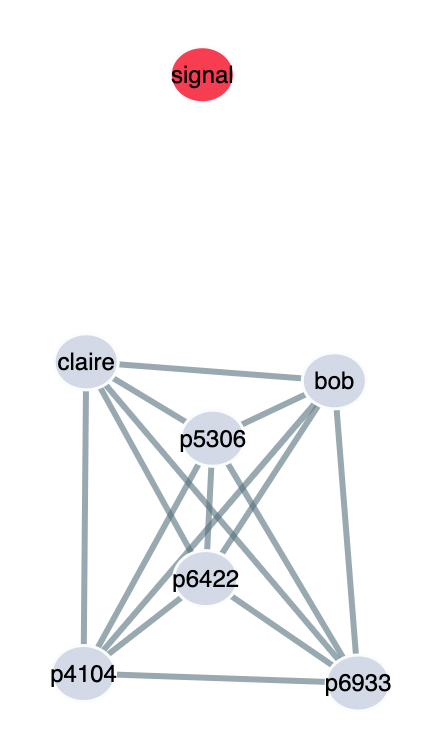
\includegraphics[width=0.25\textwidth]{graphics/analysis/mini-scenarios/lost-router/1.png} \label{fig:filmstrips-lost-router-a}}
    \subfloat[]{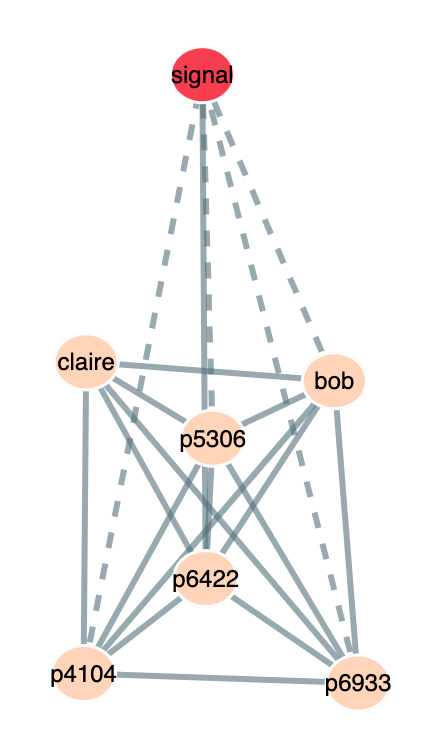
\includegraphics[width=0.25\textwidth]{graphics/analysis/mini-scenarios/lost-router/2.png} \label{fig:filmstrips-lost-router-b}}
	\subfloat[]{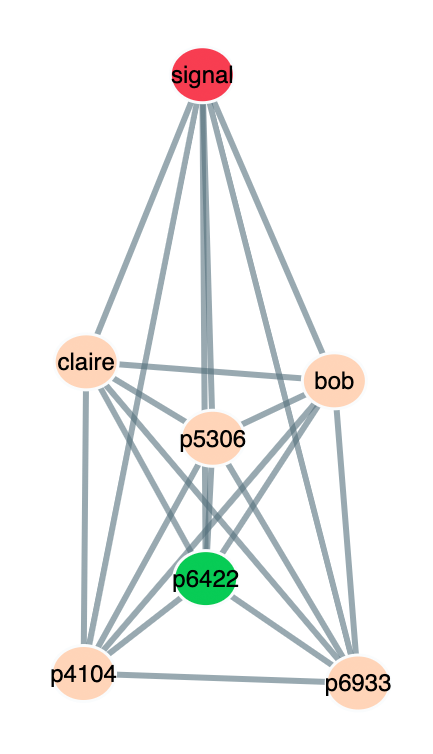
\includegraphics[width=0.25\textwidth]{graphics/analysis/mini-scenarios/lost-router/3.png} \label{fig:filmstrips-lost-router-c}}
	\subfloat[]{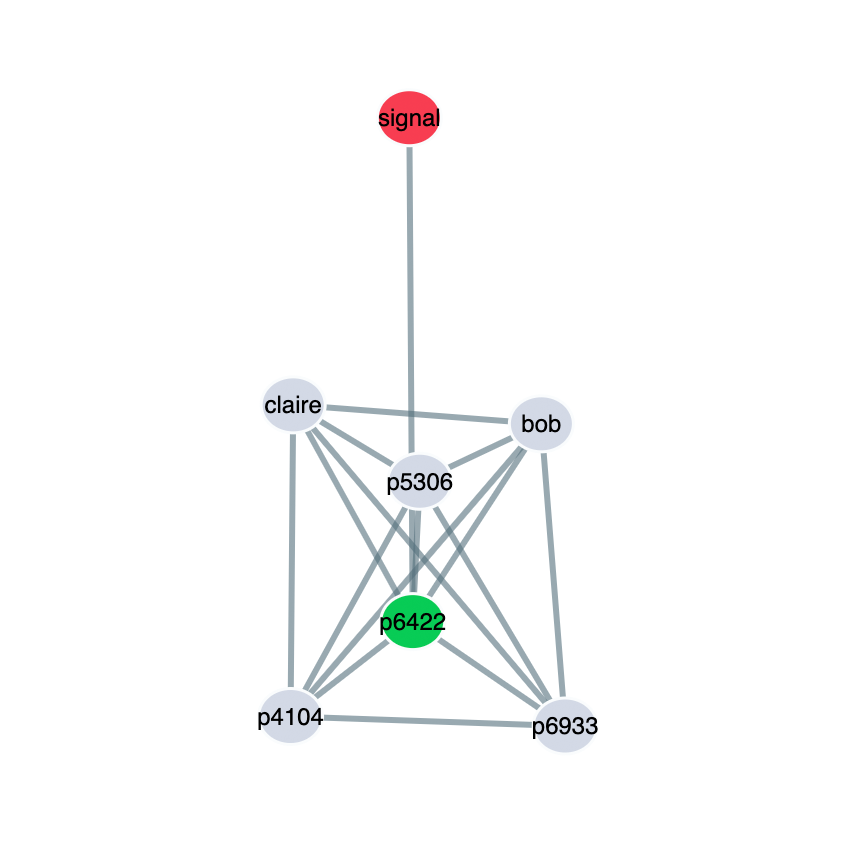
\includegraphics[width=0.25\textwidth]{graphics/analysis/mini-scenarios/lost-router/4.png} \label{fig:filmstrips-lost-router-d}}
	\caption{Router is leaving the network}
\label{fig:filmstrips-lost-router}
\end{figure}

As the peer with the role \router is a beacon for all other peers in the network, it plays an important role in the network. However, the router is not a single point of failure. It can also leave the network at any time, without causing a disruption (\vref{fig:filmstrips-lost-router-a}) in the network.

Through the LastSeen expiration mechanism, the other nodes eventually notice that there is no peer with the role \router in the network anymore. Therefore, all peers are degrading themselves to the role \newbie. Because of the \newbie role, they are contacting the \signal peer again (\vref{fig:filmstrips-lost-router-b}). As the \signal does not know any \router, it is promoting the first peer to the role \router (\vref{fig:filmstrips-lost-router-c}). Soon after the upgrade, the new \router is publishing \routerAlive messages, thus other peers notice that a router exists and close their connection to the \signal.
